\documentclass[14pt]{extbook}
\usepackage{multicol, enumerate, enumitem, hyperref, color, soul, setspace, parskip, fancyhdr} %General Packages
\usepackage{amssymb, amsthm, amsmath, latexsym, units, mathtools} %Math Packages
\everymath{\displaystyle} %All math in Display Style
% Packages with additional options
\usepackage[headsep=0.5cm,headheight=12pt, left=1 in,right= 1 in,top= 1 in,bottom= 1 in]{geometry}
\usepackage[usenames,dvipsnames]{xcolor}
\usepackage{dashrule}  % Package to use the command below to create lines between items
\newcommand{\litem}[1]{\item#1\hspace*{-1cm}\rule{\textwidth}{0.4pt}}
\pagestyle{fancy}
\lhead{Progress Quiz 9}
\chead{}
\rhead{Version B}
\lfoot{9541-5764}
\cfoot{}
\rfoot{Summer C 2021}
\begin{document}

\begin{enumerate}
\litem{
Determine the horizontal and/or oblique asymptotes in the rational function below.\[ f(x) = \frac{12x^{3} +35 x^{2} +33 x + 10}{3x^{2} +11 x + 6} \]\begin{enumerate}[label=\Alph*.]
\item \( \text{Horizontal Asymptote of } y = -3.0 \text{ and Oblique Asymptote of } y = 4x -3 \)
\item \( \text{Horizontal Asymptote of } y = 4.0 \text{ and Oblique Asymptote of } y = 4x -3 \)
\item \( \text{Horizontal Asymptote of } y = 4.0  \)
\item \( \text{Horizontal Asymptote at } y = -3.0 \)
\item \( \text{Oblique Asymptote of } y = 4x -3. \)

\end{enumerate} }
\litem{
Which of the following functions \textit{could} be the graph below?
\begin{center}
    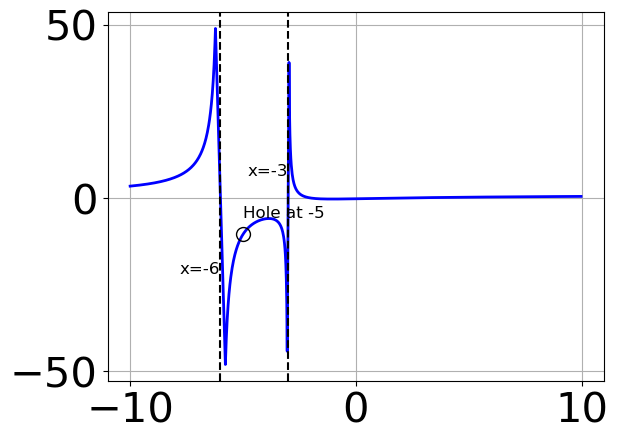
\includegraphics[width=0.5\textwidth]{../Figures/identifyGraphOfRationalFunctionCopyB.png}
\end{center}
\begin{enumerate}[label=\Alph*.]
\item \( f(x)=\frac{x^{3} + x^{2} -4.0 x -4.0}{x^{3} -14.0 x^{2} +63.0 x -90.0} \)
\item \( f(x)=\frac{x^{3} +5.0 x^{2} -4.0 x -20.0}{x^{3} +14.0 x^{2} +63.0 x + 90.0} \)
\item \( f(x)=\frac{x^{3} -5.0 x^{2} -4.0 x + 20.0}{x^{3} -14.0 x^{2} +63.0 x -90.0} \)
\item \( f(x)=\frac{x^{3} -4.0 x^{2} -4.0 x + 16.0}{x^{3} +14.0 x^{2} +63.0 x + 90.0} \)
\item \( \text{None of the above are possible equations for the graph.} \)

\end{enumerate} }
\litem{
Which of the following functions \textit{could} be the graph below?
\begin{center}
    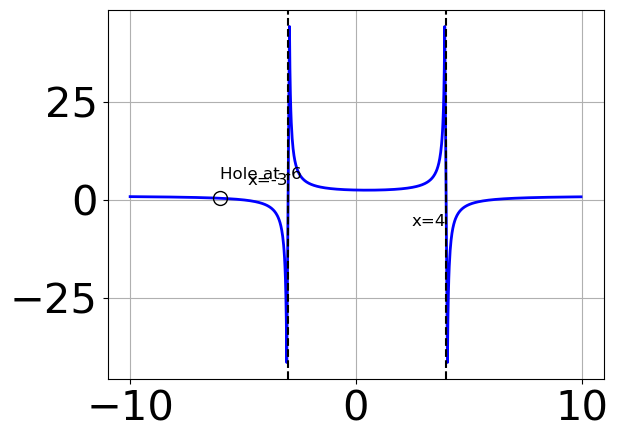
\includegraphics[width=0.5\textwidth]{../Figures/identifyGraphOfRationalFunctionB.png}
\end{center}
\begin{enumerate}[label=\Alph*.]
\item \( f(x)=\frac{x^{3} +3.0 x^{2} -34.0 x -120.0}{x^{3} +5.0 x^{2} -18.0 x -72.0} \)
\item \( f(x)=\frac{x^{3} -5.0 x^{2} -36.0 x + 180.0}{x^{3} -5.0 x^{2} -18.0 x + 72.0} \)
\item \( f(x)=\frac{x^{3} +6.0 x^{2} -25.0 x -150.0}{x^{3} -5.0 x^{2} -18.0 x + 72.0} \)
\item \( f(x)=\frac{x^{3} +5.0 x^{2} -36.0 x -180.0}{x^{3} +5.0 x^{2} -18.0 x -72.0} \)
\item \( \text{None of the above are possible equations for the graph.} \)

\end{enumerate} }
\litem{
Determine the vertical asymptotes and holes in the rational function below.\[ f(x) = \frac{12x^{3} +7 x^{2} -72 x + 45}{12x^{2} +7 x -12} \]\begin{enumerate}[label=\Alph*.]
\item \( \text{Vertical Asymptote of } x = 1.0 \text{ and hole at } x = 0.75 \)
\item \( \text{Vertical Asymptote of } x = -1.333 \text{ and hole at } x = 0.75 \)
\item \( \text{Vertical Asymptotes of } x = -1.333 \text{ and } x = 1.667 \text{ with a hole at } x = 0.75 \)
\item \( \text{Holes at } x = -1.333 \text{ and } x = 0.75 \text{ with no vertical asymptotes.} \)
\item \( \text{Vertical Asymptotes of } x = -1.333 \text{ and } x = 0.75 \text{ with no holes.} \)

\end{enumerate} }
\litem{
Determine the horizontal and/or oblique asymptotes in the rational function below.\[ f(x) = \frac{6x^{3} -1 x^{2} -72 x -80}{4x^{3} +14 x^{2} -31 x + 60} \]\begin{enumerate}[label=\Alph*.]
\item \( \text{Vertical Asymptote of } y = 4  \)
\item \( \text{Horizontal Asymptote of } y = 1.500  \)
\item \( \text{Vertical Asymptote of } y = 1.500  \)
\item \( \text{None of the above} \)
\item \( \text{Horizontal Asymptote of } y = 0  \)

\end{enumerate} }
\litem{
Determine the vertical asymptotes and holes in the rational function below.\[ f(x) = \frac{12x^{3} -79 x^{2} +144 x -80}{12x^{2} -25 x + 12} \]\begin{enumerate}[label=\Alph*.]
\item \( \text{Vertical Asymptote of } x = 1.0 \text{ and hole at } x = 1.333 \)
\item \( \text{Holes at } x = 0.75 \text{ and } x = 1.333 \text{ with no vertical asymptotes.} \)
\item \( \text{Vertical Asymptotes of } x = 0.75 \text{ and } x = 1.333 \text{ with no holes.} \)
\item \( \text{Vertical Asymptote of } x = 0.75 \text{ and hole at } x = 1.333 \)
\item \( \text{Vertical Asymptotes of } x = 0.75 \text{ and } x = 1.25 \text{ with a hole at } x = 1.333 \)

\end{enumerate} }
\litem{
Determine the horizontal and/or oblique asymptotes in the rational function below.\[ f(x) = \frac{8x^{3} -2 x^{2} -43 x + 30}{4x^{2} -23 x + 15} \]\begin{enumerate}[label=\Alph*.]
\item \( \text{Horizontal Asymptote at } y = 5.0 \)
\item \( \text{Horizontal Asymptote of } y = 2.0 \text{ and Oblique Asymptote of } y = 2x + 11 \)
\item \( \text{Oblique Asymptote of } y = 2x + 11. \)
\item \( \text{Horizontal Asymptote of } y = 5.0 \text{ and Oblique Asymptote of } y = 2x + 11 \)
\item \( \text{Horizontal Asymptote of } y = 2.0  \)

\end{enumerate} }
\litem{
Determine the horizontal and/or oblique asymptotes in the rational function below.\[ f(x) = \frac{6x^{3} +5 x^{2} -21 x + 10}{-9x^{3} +6 x^{2} +4 x -4} \]\begin{enumerate}[label=\Alph*.]
\item \( \text{Vertical Asymptote of } y = 1  \)
\item \( \text{Horizontal Asymptote of } y = 0  \)
\item \( \text{Vertical Asymptote of } y = -0.667  \)
\item \( \text{Horizontal Asymptote of } y = -0.667  \)
\item \( \text{None of the above} \)

\end{enumerate} }
\litem{
Determine the vertical asymptotes and holes in the rational function below.\[ f(x) = \frac{6x^{3} -13 x^{2} -40 x + 75}{12x^{2} -35 x + 25} \]\begin{enumerate}[label=\Alph*.]
\item \( \text{Holes at } x = 1.25 \text{ and } x = 1.667 \text{ with no vertical asymptotes.} \)
\item \( \text{Vertical Asymptotes of } x = 1.25 \text{ and } x = -2.5 \text{ with a hole at } x = 1.667 \)
\item \( \text{Vertical Asymptotes of } x = 1.25 \text{ and } x = 1.667 \text{ with no holes.} \)
\item \( \text{Vertical Asymptote of } x = 0.5 \text{ and hole at } x = 1.667 \)
\item \( \text{Vertical Asymptote of } x = 1.25 \text{ and hole at } x = 1.667 \)

\end{enumerate} }
\litem{
Determine the vertical asymptotes and holes in the rational function below.\[ f(x) = \frac{12x^{3} +37 x^{2} -59 x -60}{6x^{2} +5 x -25} \]\begin{enumerate}[label=\Alph*.]
\item \( \text{Vertical Asymptote of } x = -2.5 \text{ and hole at } x = 1.667 \)
\item \( \text{Vertical Asymptotes of } x = -2.5 \text{ and } x = -0.75 \text{ with a hole at } x = 1.667 \)
\item \( \text{Vertical Asymptotes of } x = -2.5 \text{ and } x = 1.667 \text{ with no holes.} \)
\item \( \text{Holes at } x = -2.5 \text{ and } x = 1.667 \text{ with no vertical asymptotes.} \)
\item \( \text{Vertical Asymptote of } x = 2.0 \text{ and hole at } x = 1.667 \)

\end{enumerate} }
\end{enumerate}

\end{document}